\documentclass{beamer}

\mode<presentation>
{
  \usetheme{Singapore}      
  \usecolortheme{default} 
  \usefonttheme{default}  
  \setbeamertemplate{navigation symbols}{}
  \setbeamertemplate{caption}[numbered]
} 

\usepackage[english]{babel}
\usepackage[utf8x]{inputenc}

\title[Macroprudential tools, cross-border banking and gravity]{Macroprudential policy cross-border spillovers and international banking - Any use for the gravity model?}
\author{Anni Norring}
\institute{University of Helsinki}
\date{\today}

\begin{document}

% I am going to talk about the preliminary results for a paper I'm working on with the title macroprudential policy cross-border spillovers and international banking - Any use for the gravity model?

\begin{frame}
  \titlepage
\end{frame}

\section{Introduction}

% The goal of my paper is to answer these two research questions. The first, a more general one, asks whether the gravity model of financial asset trade can tell us something about the cross-border spillovers of macroprudential policy through international banking. The second question then extends on this and asks how the implementation of macroprudential regulation in either of the countries in a bilateral pair affects the bilateral cross-border bank asset holdings. 
% Based on my preliminary results, I can state that the gravity model appears to confirm that there are spillovers through international bank lending. This is manifested through the effect of changes in the use of macroprudential instruments on cross-border bank asset holdings, which are for the most part statistically significant.

\begin{frame}{Introduction}
\begin{block}{Research questions}
\begin{itemize}
\item Can the gravity model tell us something about the cross-border spillovers of macroprudential regulation through international lending?
\item Does the implementation of macroprudential instruments in the origin country or the destination country have an effect on the bilateral cross-border bank asset holdings?
\end{itemize}
\end{block}
\begin{block}{Preliminary results}
\begin{itemize}
\item The gravity model appears to confirm that there are spillovers
\item Changes in the use of macroprudential instruments have mostly statistically significant effects on the cross-border bank asset holdings
\end{itemize}
\end{block}
\end{frame}

\section{Motivation}

% The field of research on macroprudential regulation has expanded rapidly after the introduction of macroprudential policy as a distinctive framework of economic policy after the global financial crisis. Still, there is a clear need for better understanding on the use and effectiveness of macroprudential policies. 
% Empirical multi-country studies have been very limited due to the lack of data, but there has been some improvement recently on this issue. I am using a recently published data set build and described by Cerrutti and others in 2017. This data set is the most extensive source on the use of macroprudential tools to date, and is likely to help alleviate the data limitations for its part. 
% There are also at least these two additional sources of data on the use of macroprudential tools. The first one, also by Cerrutti and others documents changes in implemented prudential tools and the second is a IMF survey that is likely to form a useful database in the future. 

\begin{frame}{Motivation for studying the use and effectiveness of macroprudential regulation}
\begin{itemize}
\item The field has been expanding rapidly, but much better understanding still needed on the use and effectiveness of macroprudential policy tools
\item Multi-country studies have been limited by the lack of data, but this no longer entirely true: 
\begin{itemize} 
\item Cerrutti et al. (2017a): The use and effectiveness of macroprudential policies: New evidence
\item Cerrutti et al. (2017b): Changes in the prudential policy instruments - A new cross-country database
\end{itemize}
\item \textbf{My contribution: combine the data from Cerrutti et al. (2017a) with data on cross-border bilateral bank asset holdings}
\end{itemize}
\end{frame}

% The implications of macroprudential policy are often not confined inside the borders of the country implementing the policy. These policies cannot be implemented in a hermetic bubble and thus some leakages and spillovers are utterly inevitable. 
% There is some, still fairly limited evidence, that the effects of macroprudential tools occasionally spill over borders through international bank lending. The meta-study of Buch and Goldberg and the papers related to this project are the most extensive look into this matter to date. The main findings of these papers are that there indeed are spillovers, but they are rather limited in nature, However, they expect the spillovers to increase in the future as more tools are taken up by more countries.
% There is also some evidence that the spillovers may reduce the effectiveness of national macroprudential policy, at least if they lead to regulatory arbitrage. Reinhardt and Sowerbutts find eviden ce of this for the UK.

\begin{frame}{Motivation for studying the cross-border spillovers of macoprudential policies}
\begin{itemize}
\item Evidence that the effects of macroprudential instruments occasionally spill over borders through international bank lending
\begin{itemize}
\item Buch and Goldberg (2017): Cross-border regulatory spillovers: How much? How important? Evidence from the International Banking Research Network, \& and the related papers
\end{itemize}
\item This may reduce the effectiveness of national macroprudential policies due to regulatory arbitrage
\begin{itemize}
\item Reinhardt and Sowerbutts (2015): Regulatory arbitrage in action: evidence from banking flows and macroprudential policy 
\end{itemize}
\item \textbf{My contribution: a multi-country look at spillovers and the effects on bilateral bank asset holdings with a large set of countries}
\end{itemize}
\end{frame}

% Why would one then use the gravity model for studying determinants of international banking? 
% Or first of all, what this gravity model even is? It was first proposed by Anderson in 1979, and it has been a workhorse model of international trade since the early eighties.
% As the name suggests, the model, inspired by elementary physics, explains a flow between two entities by simply relating it to their two masses and a friction term, which is interpreted broadly as transaction costs, which is usually proxied by the distance between the two entities. Here the gravity model is presented as log-linearized. 
%The classic gravity result is that countries tend to trade with countries that are close by, and that bilateral trade decreases as distance between the countries increases.
% In the context of international trade in financial assets, the use of the gravity model expanded rapidly after Portes and Rey first proposed it in 2005 and IMF started publishing data on bilateral portfolio investments and foreign direct investments. Portes and Rey and a multitude of papers after them found that the gravity model fits the data surprisingly well. Most of the papers confirm the classic gravity result, i.e. that as distance increases, bilateral trade decreases. "The distance puzzle" is then just another name for the classic home bias puzzle. The gravity model has since been applied to studying the determinants of foreign direct investments, M&A's and also international banking.
% The most recent example on an application to international banking is a paper published this year, by Brei and von Peter. This and other papers confirm the gravity result for banking also, i.e. that bilateral bank asset holdings decrease as the distance between the origin and destination countries increase. 

\begin{frame}{Motivation for using the gravity model of financial asset trade for international banking}
\begin{itemize}
\item The gravity model has been a workhorse of international trade literature for decades (e.g. survey by Head and Mayer, 2014)
\item The gravity model of trade in financial assets spread after Portes and Rey (2005) and IMF's CPIS-data
\item The gravity model of international banking also produces \textit{the classic gravity result}
\begin{itemize}
\item Buch (2005): Distance and international banking
\item Brei and von Peter (2018): The distance effect in banking and trade
\end{itemize}
\item \textbf{My contribution: using the gavity model for studying the spillovers from macroprudential policy}
\begin{itemize}
\item With a clear emphasis on macroprudential regulation, differing from Houston et al. (2012): Regulatory arbitrage and international bank flows
\end{itemize}
\end{itemize}
\end{frame}


\section{Goal of this paper}

% ON THIS SLIDE: WHAT IT THE CONTRIBUTION OF MY PAPER?

\begin{frame}{Goal of this paper}
\begin{itemize}
\item Consider in parallel new data on macroprudential instruments and bilateral cross-border bank asset holdings
\item Provide a multi-country look at the spillovers of macroprudential policy via international lending with a set of countries larger than in previous studies
\item Use the gravity model of international banking to study the effects of macroprudential policy that leak across borders via international lending
\end{itemize}
\textit{... in order to answer...}
\begin{itemize}
\item Can the gravity model tell us something about the cross-border spillovers of macroprudential regulation through international lending?
\item Does the implementation of macroprudential instruments in the origin country or the destination country have an effect on the bilateral cross-border bank asset holdings?
\end{itemize}
\end{frame}

\section{Data}

%For the independent variable of interest, the use of macroprudential tools, I make use of a recently published data set called the Global Macroprudential Instruments Survey. This data is described in the Cerrutti et al 2017 paper. It is an annual index for the years 2000 to 2013 (so the data itself is not that recent unfortunately) and it is collected by the IMF. The coverage is 119 countries, and 117 of these are either BIS LBS reporting countries or counterparty countries to BIS reporting countries. 
% The data is quite extensive, it covers almost 20 different tools, of which 10 are aggregated into an aggregate index on tools that target financial institutions and 2 into an index on tools that target borrowers. Thus the structure of these indices fit my hypotheses perfectly. 
% There are caveats. The indices are based on survey data and cover years when the macroprudential framework was non-existent or just beginning to take shape. Also the details of each tools vary from country to country. Thus consistency is a big issue that needs to be kept in mind when interpreting the results. 

\begin{frame}{Data: The use of macroprudential instruments}
\begin{itemize}
\item From the IMF Global Macroprudential Instruments Survey
\item Annual index for 2000-2013
\item 119 countries, 117 of which are BIS reporting countries or counterpart countries to BIS reporting countries 
\item Data includes two aggregate indices: for instruments targeting financial institutions ($mpif$) and those targeting borrowers ($mpib$)
\begin{itemize}
\item $mpif$ aggregates 10 tools that include e.g. different capital requirements, limits on interbank exposures, loan growth, leverage ratio etc.
\item $mpib$ aggregates 2 tools; LTV-ratio and DTI-ratio
\end{itemize}
\item Described in Cerrutti et al. (2017a) and used to show that there is a link between slower credit growth and the use of macroprudential policy
\end{itemize}
\end{frame}

%The most important thing to note about the indices is that they do not even try to account for the relative differences in how stringent the regulation is, simply if a tool has been implemented. Thus the index changes in exactly the same way for a country that implements a 0.1% countercyclical capital buffer and a country that implements a 5% one. Also, the indices do not distinguish between a binding regulation and a recommendation, and if the stance of an already implemented tool is tightened, the index does not budge. 
% From table 3 it's easy to note, that even though prudential tools are quite widely used, by all means not all countries implement prudential regulation. 

\begin{frame}{Data: The use of macroprudential instruments}
\begin{table}[!h]
\centering
\begin{tabular}{ l l l l l l l }
\hline
Variable&Mean&Std. dev.&Min&Max&Range&Obs. \\
\hline
$mpif$&1.38&1.24&0&6&0-10&1 638 \\
$mpib$&0.36&0.66&0&2&0-2&1 638 \\
\hline
\end{tabular}
\caption{Macroprudential indices targeting financial institutions and borrowers}
\label{tab:mpi}
\end{table}

\begin{table}[!h]
\small
\centering
\begin{tabular}{ l l l l l l l l l }
\hline
Value&0&1&2&3&4&5&6&7-10\\
\hline
$mpif$&28.9\%&29.9\%&23.8\%&11.7\%&3.7\%&1.7\%&0.4\%&- \\
$mpib$&74.6\%&15.3\%&10.2\%&-&-&-&-&- \\
\hline
\end{tabular}
\caption{Use of macroprudential tools: \% of all observations with n tools implemented}
\label{tab:mpiu_use}
\end{table}
\end{frame}

%My dependent variable is bilateral cross-border bank asset holdings from the BIS locational banking statistics. To extend the coverage of the data, I lay data on assets and liabilities over each other, in order to build a network of bilateral holdings for pairs of countries where both are BIS reporting countries or where either the origin country or the destination country is a BIS reporting country. This extends the coverage beyond just taking the asset data, and it is quite surprising that Brei and von Peter can claim to be the first to have overlaid the data this way, because it was a rather simple exercise. A side note: the publicly available locational banking statistics is not very useful because so much of these bilateral observations are confidential. I however have all the data, as I had access to it when I was at the Bank of Finland, so confidentiality is not an issue. 
% Draw the matrix of data on white board

\begin{frame}{Data: The dependent variable}
\begin{block}{Bilateral cross-border bank asset holdings}
\begin{itemize}
\item From BIS Locational Banking Statistics
\item I build a network of bilateral holdings for pairs of origin countries and destination countries that are both BIS reporting countries or where either the origin country or the destination country is a BIS reporting country (following Brei and von Peter, 2018):
\begin{itemize}
\item O reports to BIS: use data on assets
\item O does not report to BIS, but D does: use data on liabilities
\item Neither O nor D reports to BIS: missing value
\end{itemize}
\item Maximum coverage: 44 reporting countries, 216 counterpart countries and quarterly data since 1977
\item For the purpose of this paper: 33 reporting countries, 84 counterpart countries and annual data for 2000-2013
\end{itemize}
\end{block}
\end{frame}

%Here are some summary statistics on the dependent variable. The data is in dollars, and there is a lot of variation. The minimum value is 0 in my sample, but in the full sample there were eight negative observations, which I have dropped. These were not at least necessarily mistakes, but the stock of holdings can be negative due to short selling.
%Noteworthy is the share of zero observations, which is very large, almost 45 %. This is a common feature of all bilateral data, in trade, in portfolio investing and in banking. It is also an important driver of the results and calls for the use of estimation methods that are suitable for limited dependent variables. 

\begin{frame}{Data: The dependent variable}
\begin{table}
\tiny
\centering
\begin{tabular}{l|r r r r}
\hline
 & $ba_{od}$ & $ba_{od} > 0$ & $log(ba_{od} + 1)$ & $log(ba_{od})$ \\ 
\hline
N of pairs & 6 112 & 4 674 & 6 112 & 4 674 \\
N of periods & 14 & 14 & 14 & 14 \\
N of observations & 85 560 & 51 013 & 85 560 & 51 013 \\
\hline
%Unit & \multicolumn{4}{l}{Thousands of US dollars} \\
%\hline
Mean & 6 277 587 & 11 281 030 & 6.73 & 12.10 \\
Standard deviation & 56 285 910 & 75 081 810 & 6.45 & 3.12 \\
Min & 0 & 0.01 & 0 & 2.30\\
Max & 2 962 748 000 & 2 962 748 000 & 21.81 & 21.81 \\
\hline
Share of 0s & 44.35 \% & - & 44.35 \% & -  \\
\hline 
\multicolumn{5}{l}{\tiny Mean, standard deviations, min and max in thousands of US dollars.}
%Number of pairs & \multicolumn{3}{l}{test}\\
\end{tabular}
\caption{Summary statistics of the dependent variable.}
\label{tab:ba_od}
\end{table}
\end{frame}



%The sources for the data for the other independent variables are listed here. The economic masses are annual GDP from the World Bank. I gave a similar presentation at the Bank of Finland last week, and they suggested that in this case proxying the economic mass with the size of the banking sector, at least in the origin country, might be sensible also, at least as a robustness check, but this I'm still working on. 
%The different friction controls are mostly taken from the CEPII gravity database. I use a population-weighted distance instead of just a simple geographical distance between capitals. The gravity literature uses a very imaginative myriad of different controls, but I've chosen the ones most commonly used and found to have statistically significant effects. In addition to the classic gravity frictions, I control for financial sophistication with four different variables. 
%In the gravity literature, the need to control for a so called multilateral resistance term is emphasized. This is meant to capture the fact that the assets of any given country must "compete" with the assets of all the other countries. This term is often proxied by regional dummies, which is the approach I have taken. They could also be proxied by country fixed effects on the pairs, or all the origin countries and the destination countries. In addition there are time fixed effects taken into account. 

\begin{frame}{Data: Other independent variables}
\begin{block}{Economic mass}
\begin{itemize}
\item Annual GDP from World Bank
\item \textit{Size of the banking sector?}
\end{itemize}
\end{block}
\begin{block}{Frictions, data from CEPII's gravity database}
\begin{itemize}
\item Population-weighted distance
\item Gravity controls: contiguity, common language, common colonial history, common currency
\item Financial sophistication: income group, financial openness, membership in the WTO, membership in the EU
\end{itemize}
\end{block}
\begin{block}{Other controls}
\begin{itemize}
\item Time fixed effects, country fixed effects or a regional dummy
\end{itemize}
\end{block}
\end{frame}

\section{Model}

%Let's then move on to the gravity model itself. Here I have first the most simple form of the log-linearized gravity equation. This equation relates the log of bilateral assets to the logs of the respective economic masses and a friction term tau, which represents transaction costs. In the most simple versions of the model these costs are simply proxied by the bilateral distance. 
%Usually however more bells and whistles are added to the equation. It is common to control for different frictions by adding say different variables that account for frictions in information transmission and in transaction technology. The multilateral resistance term is often proxied by regional dummies. It is also common to control for macroeconomic conditions by using time fixed effects. 

\begin{frame}{The gravity model of financial asset trade}
\textbf{The gravity equation in the most simple form:}
\begin{align}
log(asset_{od,t}) = & \alpha_1 log(M_{o,t}) + \alpha_2 log(M_{d,t})  \nonumber \\
& + \alpha_3 log(\tau_{od,t}) + u_{od,t}, \\
& o, d=1, ..., N \text{ and } t=1, ..., T. \nonumber
\label{simple gravity}
\end{align}
\textbf{The gravity equation in the form often estimated:}
\begin{align}
log(asset_{od,t})= & \alpha_1 log(GDP_{o,t})+\alpha_2 log(GDP_{d,t}) +\alpha_3 log(dist_{od}) \nonumber\\
& + \text{information variables} \nonumber\\
& + \text{transaction technology variables}\nonumber\\
& + \text{multilateral resistance} + \text{time dummies} \nonumber\\
& + \text{constant}+ u_{od,t},  \\
& o, d=1, ..., N \text{ and } t=1, ..., T. \nonumber
\label{usual gravity}
\end{align}
\end{frame}

%For the purpose of this paper I formulate the gravity equation like this. The dependent variable is the log of bilateral banking assets, held by banks in origin country with destination country as the counterpart. The economic masses are represented by GDP in logs. Distance is also in logs. 
%I basically add this second row in to the equation, that is I have four variables that account for the use of prudential tools in the two countries. First is the use of tools that target borrowers in the origin country, second the use of tools that target borrowers in the destination countries. Third and fourth document the use of prudential tools that target financial institutions in the origin and destination country respectively. 
%Then I include the most common gravity controls and controls for financial sophistication in both countries. I proxy multilateral resistance by using regional dummies, and include time dummies to account for macroeconomic conditions. 
%There are 117 origin and destination countries, which makes up over 6000 bilateral pairs. The time runs from 1 to 14, i.e. from 2000 to 2013. 

\begin{frame}{The gravity model for the purpose of this paper}
\begin{align}
log(ba_{od,t})= & \alpha_1 log(GDP_{o,t})+\alpha_2 log(GDP_{d,t}) +\alpha_3 log(distw_{od}) \nonumber\\
& + \alpha_4 mpif_{d,t} + \alpha_5 mpif_{o,t} + \alpha_6 mpib_{d,t} + \alpha_7 mpib_{o,t} \nonumber\\
& + \text{gravity controls} \nonumber\\
& + \text{controls for financial sophistication} \nonumber\\
& + \text{multilateral resistance} \nonumber\\
& + \text{time dummies} \nonumber\\
& + \text{constant}+ u_{od,t},  \\
& o, d=1, ..., 117 \text{ and } t=1, ..., 14. \nonumber
\label{my gravity}
\end{align}
\end{frame}

%Let's next consider the hypotheses in a bit more detail to better fit them into the bilateral gravity framework. Recall first that I had to hypotheses: one concerning regulation aimed at financial institutions and one for regulation aimed at borrowers. The important assumption here underpinning the different effects of these regulations is that they differ in scope.

\begin{frame}{Hypotheses in more detail}
\begin{block}{Hypotheses - regulations differ} 
\begin{itemize}
\item \textbf{Tightening capital requirements for financial institutions} leads to domestic agents borrowing more abroad 
\item \textbf{Tightening regulation that applies to domestic borrowers} does not lead to more borrowing from abroad, but instead banks might move lending to less regulated markets
\end{itemize}
\end{block}
\end{frame}

%Regulation aimed at making financial institutions more resilient is often applicable only to domestic banks and foreign subsidiaries, but not foreign branches. This means that tighter regulation in a given country creates a funding advantage for foreign banks. In the two-way set-up of the gravity framework this would mean that:
%Tighter regulation in the destination country leads to higher banking flows from the origin to the destination as banks from the origin country take advantage of the funding differential. Thus a higher mpif index for destination country is expected to be associated with more cross-border lending.
%On the other hand, tighter regulation in the origin country creates a funding advantage for foreign banks, increasing competition in the domestic market. This may lead to lower banking flows from origin country to destination country if banks from the origin reduce cross-border activity to better comply with regulation and to take on increased competition. Thus a higher mpif index for origin country is expected to be associated with less cross-border lending. 

\begin{frame}{Hypotheses in more detail}
\begin{block}{Tightening capital requirements for financial institutions}
\begin{itemize}
\item Regulation that applies to domestic banks and foreign subsidiaries, but not foreign branches
\item Tighter regulation in the destination country leads to higher banking flows from O to D as banks from the origin country take advantage of a funding differential
\begin{itemize}
\item a higher $mpif_{d}$ is associated with a higher $ba_{od}$
\end{itemize}
\item Tighter regulation in the origin country may lead to lower banking flows from O to D as banks from the origin country reduce cross-border activity to better comply with the more stringent regulation
\begin{itemize}
\item a higher $mpif_{o}$ is associated with a lower $ba_{od}$
\end{itemize}
\end{itemize}
\end{block}
\end{frame}

%The regulation aimed at domestic borrowers, because of say worryingly high growth in leverage growth, works differently, because it applies to domestic agents and via them to all banks operating in the domestic market. Now there is no funding advantage for any banks, and there is no effect on international lending through this channel. However, tighter regulation can still spill over, if banks retreat from a more regulated market to a less regulated one. Then
%tighter regulation in the destination country leads to lower banking flows as banks from the origin country retreat from a more heavily regulated market. Thus a higher mpib index for the destination country is associated with lower banking flows from o to d.
%Conversely, tighter regulation aimed at borrowers in the origin country would then be expected to lead to higher banking flows as banks from the origin country move to less regulated markets, as a clear instance of regulatory arbitrage. I.e. a higher mpib index for the the origin country is associated with higher banking flows. 
% To be completely frank, these hypotheses are not consistently confirmed in the estimations. This may be because of the different uncertainties and peculiarities of the data, the highly non-linear model or then the channels of effect are somehow different. If you have some idea for how they could be different, I would be happy to discuss it. 

\begin{frame}{Hypotheses in more detail}
\begin{block}{Tightening regulation that applies to domestic borrowers}
\begin{itemize}
\item Regulation that applies to all banks operating in the country
\item Tighter regulation in the destination country leads to lower banking flows from O to D as banks from the origin country retreat from a more heavily regulated market
\begin{itemize}
\item a higher $mpib_{d}$ is associated with a lower $ba_{od}$
\end{itemize}
\item Tighter regulation in the origin country leads to higher banking flows from O to D as banks from from the origin country move lending to less regulated markets (regulatory arbitrage)
\begin{itemize}
\item a higher $mpib_{o}$ is associated with a higher $ba_{od}$
\end{itemize}
\end{itemize}
\end{block}
\end{frame}


\section{Estimation}

%There are a number of different estimation methods to be used to estimate the gravity equation. The most simple one has also been the most commonly used: a panel fixed effects OLS with zero observations excluded by taking log. This is however a very simplistic approach because as with any bilateral data, the share of zeros is usually very high. The problem of zero observations is usually acknowledged but then ignored by the early gravity papers. 
%The method that is perhaps on the most firm theoretical footing is the one proposed by Santos Silva and Tenreyro: the Poisson pseudo-maximum-likelihood (PPML). This method doesn't require the model to be log-linearized, so there is no problem of loosing out on the zero observations. 
%One more method I have ran into was proposed by Drakos and others in 2014. Their idea is to take the dependent variable, portfolio investments in their case, as dichotomous, i.e. taking value 1 if the investment holding is positive and zero otherwise. This allows them to use a panel probit and also to consider a dynamic version of the model. Their approach however is unable to say anything about the determinants of the level of investment holdings.
%My choice is not the PPML, but instead a different way to address the limited nature of my dependent variable. This estimation method is called the double-hurdle model and it was first proposed by Cragg in the early seventies and developed further by Heckmann. This model ensures an appropriate treatment of zero observations and it considers zeros as true zeros, that is not as missing values as the sample selection model does. An additional feature of the model is that allows for breaking the problem into two equation: a participation equation that estimates the determinants of the dependent variable being positive and a level equation which estimates the determinants of the level of the dependent variable, given that it is positive. The decision to invest in a foreign country or to extend credit to foreign borrowers, is intuitively quite easy to separate into these different stages of decision making, thus adding to the double-hurdle model's appeal. Now a Tobit model can do this, but what really makes the double-hurdle model interesting is that it allows for the two processes to be different. The size of the coefficients, or their sign can be different in the two equations, even the independent variables can be different altogether. A classic example of the power of the double-hurdle model is the effect of education on smoking: a more educated person is less likely to smoke, i.e. the coefficient is negative in the participation equation, but given that a person smokes, a more educated person is likely to smoke more, i.e. the coefficient is positive in the level equation. 

\begin{frame}{Possible estimations methods}
\begin{itemize}
\item Panel fixed effects OLS with zero observations excluded (e.g. Portes and Rey, 2005)
\item Poisson pseudo-maximum-likelihood (PPML) approach (proposed by Santos Silva and Tenreyro, 2006)
\item Panel probit with a dichotomous dependent variable (proposed Drakos et al., 2014)
\item My choice: the double-hurdle model
\begin{itemize}
\item A method first proposed by Cragg (1971) and developed further by Heckman (1976)
\item Ensures an appropriate treatment of zero observations
\item Breaks the equation into a participation equation and a level equation
\item \textbf{Both parts can be determined by different processes}, i.e. an extension to Tobit
\end{itemize}
\end{itemize}
\end{frame}

%From this simple scatter plot, it is quite easy to argue for the use of the double-hurdle model. Recall that 45 % of all observations are zero. Then simply from eyeballing this graph one can see that the relationship between the bilateral banking asset holdings and distance would not be nearly as negative. 

\begin{frame}{Why the double-hurdle?} 
\begin{figure}
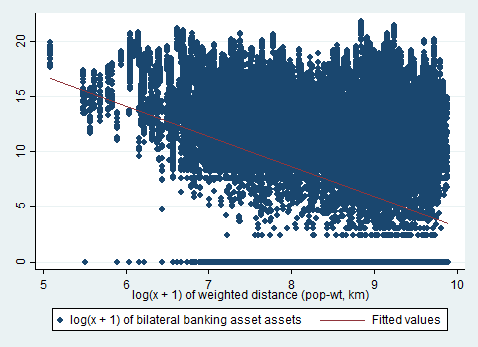
\includegraphics[width=\textwidth]{scatter_lfit_log1_ba_od_log1_distw.png}
\caption{\label{fig2}The observations obtained from the BIS LBS data.}
\end{figure}
\end{frame}

\begin{frame}{Why the double-hurdle?} 
\begin{figure}
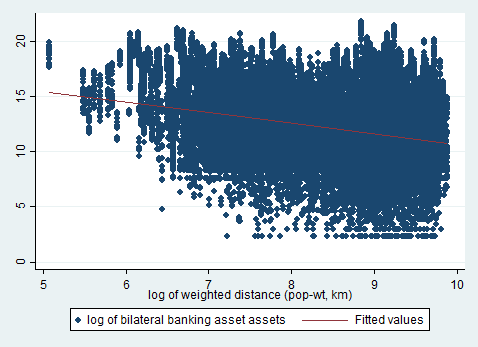
\includegraphics[width=\textwidth]{scatter_lfit_log_ba_od_log_distw.png}
\caption{\label{fig2}The observations obtained from the BIS LBS data.}
\end{figure}
\end{frame}

\begin{frame}{Why the double-hurdle?} 
\begin{table}[!h]
\tiny
\centering
\begin{tabular}{ l | c  c  c }
&Probit (depvar $dba_{od}$) &FE OLS (depvar $log(ba_{od})$) \\
\hline
$log(GDP_{o})$&0.108****&0.356****&\\
&(0.002)&(0.109)&\\
$log(GDP_{d})$&0.128****&1.385****&\\
&(0.002)&(0.110)&\\
$log(distw_{od})$&-0.229****&-1.104****&\\
&(0.006)&(0.050)&\\
$mpif_{d}$&-0.008*****&-0.026&\\
\textbf{effect positive} &(0.002)&(0.017)&\\
$mpif_{o}$&\textbf{-0.008}****&\textbf{-0.046}***&\\
\textbf{effect negative} &(0.002)&(0.018)&\\
$mpib_{d}$&0.012****&0.056**&\\
\textbf{effect negative} &(0.003)&(0.026)&\\
$mpib_{o}$&\textbf{0.013}****&\textbf{0.068}**&\\
\textbf{effect positive} &(0.003)&(0.030)&\\
$$&&\\
%&()&()&()&()&()&()\\
gravity controls &Yes&Yes \\ 
financial soph. ctrls &Yes&Yes \\
regional &Yes&Yes \\
\hline
\multicolumn{3}{l}{\tiny Significance at the 10\%, 5\%, 1\% and 0.1\% levels is }\\
\multicolumn{3}{l}{\tiny Sdenoted by *, **, *** and **** respectively.}\\
\multicolumn{3}{l}{\tiny Standard errors in parentheses.}\\
\multicolumn{3}{l}{\tiny The effects that are in line with hypotheses are bolded.}\\
\end{tabular}
\caption{Average marginal effects and hypotheses}
\label{tab:methods}
\end{table}
\end{frame}



%The equation I estimate is thus this one. In the first specification I include only the economic masses, distance and the macroprudential variables. To the second specification I add the gravity and financial sophistication controls and to the third also the regional dummies proxying multilateral resistance. Time dummies and a constant are included in all the specifications.
%The first hurdle in the double hurdle estimates the effect of independent variables on the probability of bilateral bank asset holdings being positive. This equation is estimated using probit.
%The level equation, or the second hurdle estimates the effect of a change on the level of bilateral banking assets conditional on the level being positive. 
%According to the previous results on gravity equations alpha1 and alpha 2 should be positive and alpha 3 negative. This is indeed the case for all specifications. According to my hypotheses alpha 4 and and alpha 7 should be positive, and alpha 5 and alpha 6 should be negative, and this is the case half the time.

\begin{frame}{The equation to be estimated}
\begin{align}
log(ba_{od,t})= & \alpha_1 log(GDP_{o,t})+\alpha_2 log(GDP_{d,t}) +\alpha_3 log(distw_{od}) \nonumber\\
& + \alpha_4 mpif_{d,t} + \alpha_5 mpif_{o,t} + \alpha_6 mpib_{d,t} + \alpha_7 mpib_{o,t} \nonumber\\
& + \text{gravity controls} \nonumber\\
& + \text{controls for financial sophistication} \nonumber\\
& + \text{multilateral resistance term} \nonumber\\
& + \text{time dummies} \nonumber\\
& + \text{constant}+ u_{od,t},  \\
& o, d=1, ..., 117 \text{ and } t=1, ..., 14. \nonumber
\label{my participation}
\end{align}
\begin{itemize}
\item \textbf{The participation equation:} the effect of independent variables on the probability of $ba_{od,t}$ being positive
\item \textbf{The level equation:} the effect of a change in independent variables on the level of $ba_{od,t}$ conditional on the level being positive
\end{itemize}
\end{frame}

\section{Results}

%For some reason running the double-hurdle on stata is horribly slow, so estimating these three specifications and calculating the needed marginal effects takes about three days. So after stata has been crunching numbers for some 72 hours, I get these marginal effects. The effects for the participation equation tell the effect a change in the independent variable has on the probability of the dependent variable being positive. The effects for the level equation tell the effect a change in the independent variable has on the level of the dependent variable, conditional on it being positive. 
%What I found surprising about these effects is that they are practically all highly statistically significant. I would have expected that the effects for at least mpif_o to be less significant. I'm as of yet at least unable to say if this because these indices pick something that I should control in some other way, or if there is a bad endogeneity problem or something going on. This is something I should work on to really try to understand what's going on here.

%As I said before, my hypothesis are not consistently backed up by the results. Here I have in bold font the effects that are consistent with the hypothesis, and we can see that exactly half of the effects are of the sign I expected, but interestingly, even this is not consistent. So it's not so that all effects of say mpif_o are of the expected sign and all of mpif_d are not. So it's quite clear that some work is required to think the hypotheses and the channels of effect through clearly to build a coherent story of what's going on there. 

\begin{frame}{Marginal effects and hypotheses}
\tiny
\begin{table}[!h]
\centering
\begin{tabular}{ l l l l l}
\hline
Specification&(1)&&(2)& \\
Depvar: $log(ba_{od}+1)$&Participation&Level&Participation&Level\\
\hline
$log(GDP_{o}+1)$&0.08****&0.59****&0.08****&0.62****\\
&(0.00)&(0.01)&(0.00)&(0.01)\\
$log(GDP_{d}+1)$&0.09****&0.60****&0.09****&0.61****\\
&(0.00)&(0.01)&(0.00)&(0.01)\\
$log(distw_{od}+1)$&-0.16****&-0.81****&-0.10****&-0.88****\\
&(0.00)&(0.01)&(0.00)&(0.01)\\
$mpif_{d}$&-0.01****&-0.17****&\textbf{0.02}****&-0.10****\\
\textbf{effect positive}  &(0.00)&(0.01)&(0.00)&(0.01)\\
$mpif_{o}$&\textbf{-0.02}****&\textbf{-0.17}****&0.02****&\textbf{-0.09}****\\
\textbf{effect negative} &(0.00)&(0.01)&(0.00)&(0.01)\\
$mpib_{d}$&0.03****&0.28****&\textbf{-0.02}****&\textbf{-0.25}****\\
\textbf{effect negative} &(0.00)&(0.02)&(0.00)&(0.01)\\
$mpib_{o}$&\textbf{0.02}****&\textbf{0.32}****&-0.00&-0.14****\\
\textbf{effect positive} &(0.00)&(0.02)&(0.00)&(0.01)\\
$$&&&&\\
%&()&()&()&()&()&()\\
gravity controls &No&No&Yes&Yes \\ 
financial soph. ctrls &No&No&Yes&Yes \\
regional &No&No&Yes&Yes \\
\hline
\multicolumn{5}{l}{\tiny Significance at the 10\%, 5\%, 1\% and 0.1\% levels is denoted by *, **, *** and **** respectively.}\\
\multicolumn{5}{l}{\tiny Standard errors in parentheses.}\\
\multicolumn{5}{l}{\tiny The effects that are in line with hypotheses are bolded.}\\
\end{tabular}
\caption{Average marginal effects and hypotheses}
\label{tab:results}
\end{table}
\end{frame}

%In this table I have the marginal effects of either a percent change in the log-variables or a unit change in the integer variables interpreted as percent changes on the probability of dependent variable being positive and on the level of positive holdings. 
%I find some of these effects to be surprisingly large, and would be careful of putting too much weight on the size of these effects at least before proper robustness checks. Some of these feel quite believable, say the 2 % increase in probability of a positive level of international lending after one unit increase in mpib_o, but that the level of positive lending should increase 32 % is quite doubtful, even without considering that these effects change a lot across the three specifications. 
%It is not however unheard of to fund these average marginal effects on bilateral flows or holdings to be very large. So this might in fact reflect some bias in the gravity model, perhaps due to estimating it in the log-linearized form. Thus using the PPML method at least as a robustness check would probably be very sensible. 

\begin{frame}{Interpreting the marginal effects}
\tiny
\begin{table}[!h]
\centering
\begin{tabular}{ l l l l l}
\hline
Specification&(1)&&(2)& \\
Depvar: $log(ba_{od}+1)$&Participation&Level&Participation&Level\\
\hline
$log(GDP_{o}+1)$, \%-change&0.08\%&0.59\%&0.08\%&0.62\%\\
$$&&&&\\
$log(GDP_{d}+1)$, \%-change&0.09\%&0.60\%&0.09\%&0.61\%\\
$$&&&&\\
$log(distw_{od}+1)$, \%-change&-0.16\%&-0.81\%&-0.10\%&-0.88\%\\
$$&&&&\\
$mpif_{d}$, unit change&-1\%&-17\%&\textbf{2\%}&-10\%\\
\textbf{effect positive}  &&&&\\
$mpif_{o}$, unit change&\textbf{-2\%}&\textbf{-17\%}&2\%&\textbf{-9\%}\\
\textbf{effect negative} &&&&\\
$mpib_{d}$, unit change&3\%&28\%&\textbf{-2\%}&\textbf{-25\%}\\
\textbf{effect negative} &&&&\\
$mpib_{o}$, unit change&\textbf{2\%}&\textbf{32\%}&\textit{-0\%}&-14\%\\
\textbf{effect positive} &&&&\\
$$&&&&\\
%&()&()&()&()&()&()\\
gravity controls &No&No&Yes&Yes \\ 
financial soph. ctrls &No&No&Yes&Yes \\
regional &No&No&Yes&Yes \\
\hline
\multicolumn{5}{l}{\tiny Significance at the 10\%, 5\%, 1\% and 0.1\% levels is denoted by *, **, *** and **** respectively.}\\
\end{tabular}
\caption{The percent changes in the dependent variable associated with a change in controls}
\label{tab:percentchange}
\end{table}
\end{frame}

\section{Conclusions}

%I would thus conclude by saying that yes, it indeed appears to be the case that the gravity model can be of use in estimating the spillovers and leakages of macroprudential regulation. There is however need for further robustness checks, perhaps using different estimation methods. The results from the double-hurdle model emphasize the need to be very careful in interpreting the results. 
%The estimation results point to there being statistically significant marginal effects and that these may be non-negligible. As such my result support the findings that there are cross-border spillovers of macrprudential regulation, but I would not be confident enough to use the exact numbers of percent changes just yet. 

\begin{frame}{Conclusions}
\begin{block}{Can the gravity model tell us something about the cross-border spillovers of macroprudential regulation through international lending?}
\begin{itemize}
\item This indeed appears to be the case
\item Need for robustness checks using different estimation strategies
\item Results should be interpreted very carefully
\end{itemize}
\end{block}
\begin{block}{Does the implementation of macroprudential instruments in the origin country or the destination country have an effect on the bilateral cross-border bank asset holdings?}
\begin{itemize}
\item There appears to be statistically significant marginal effects and they may be non-negligible
\item Support for there being significant cross-border spillovers of macroprudential regulation
\end{itemize}
\end{block}
\end{frame}

\begin{frame}
\begin{center}
\textbf{Thank you!}
\vskip 1cm
All comments and suggestions are warmly welcome: \\
anni.norring@helsinki.fi
\end{center}
\end{frame}

\begin{frame}{References}
\begin{itemize}
\item Avdjiev, S., Koch, C., McGuire, P., von Peter, G., 2017. International prudential spillovers: a global perspective. International Journal of Central Banking, Vol. 13, No. S1.
\item Brei, M., von Peter, G., 2018. The distance effect in banking and trade. Journal of International Money and Finance, 81, 116-137.
\item Buch, C., Goldberg, L. (2016). “Cross-border prudential policy spillovers: How much? How important? Evidence from the international banking research network”. NBER Working Paper 22874.
\item Cerutti, E., Claessens, S., Laeven, L., 2017. “The use and effectiveness of macroprudential policies: New evidence”. Journal of Financial Stability, 28 (2017) 203-224.
\item Cerrutti, E., Correa, R., Fiorentino, E., Segalla, E., 2017. “Changes in Prudential Policy Instruments - A New Cross-Country Database,” International Journal of Central Banking 13.
\item Reinhardt, D. and Sowerbutts, R., 2015. “Regulatory arbitrage in action: evidence from banking flows and macroprudential policy”. Bank of England Staff Working Paper No. 546.
\end{itemize}
\end{frame}

\end{document}

